\chapter{Spanning Tree Protocol (STP)}

\section{Switch Manual}
The user manual for the switch is available here:

\url{http://www.jaumebarcelo.info/teaching/lxs/stp/manual_spantree.pdf}

\section{Introduction}

In this assignment you will configure the Spanning Tree Protocol (STP). This protocol is used in Ethernet networks to establish which are the active link and therefore which is the path that data packets will follow. The switches that you will use are the same as the ones in the previous assignment. Have your VLAN report handy just in case you need to consult it and to remember which are the basic commands to interact with the switch.

\section{Theoretical Construction of the Tree}

The switches are connected as illustrated in the figure \ref{fig:StpTopology}.

\begin{figure}
\centering
\ifpdf
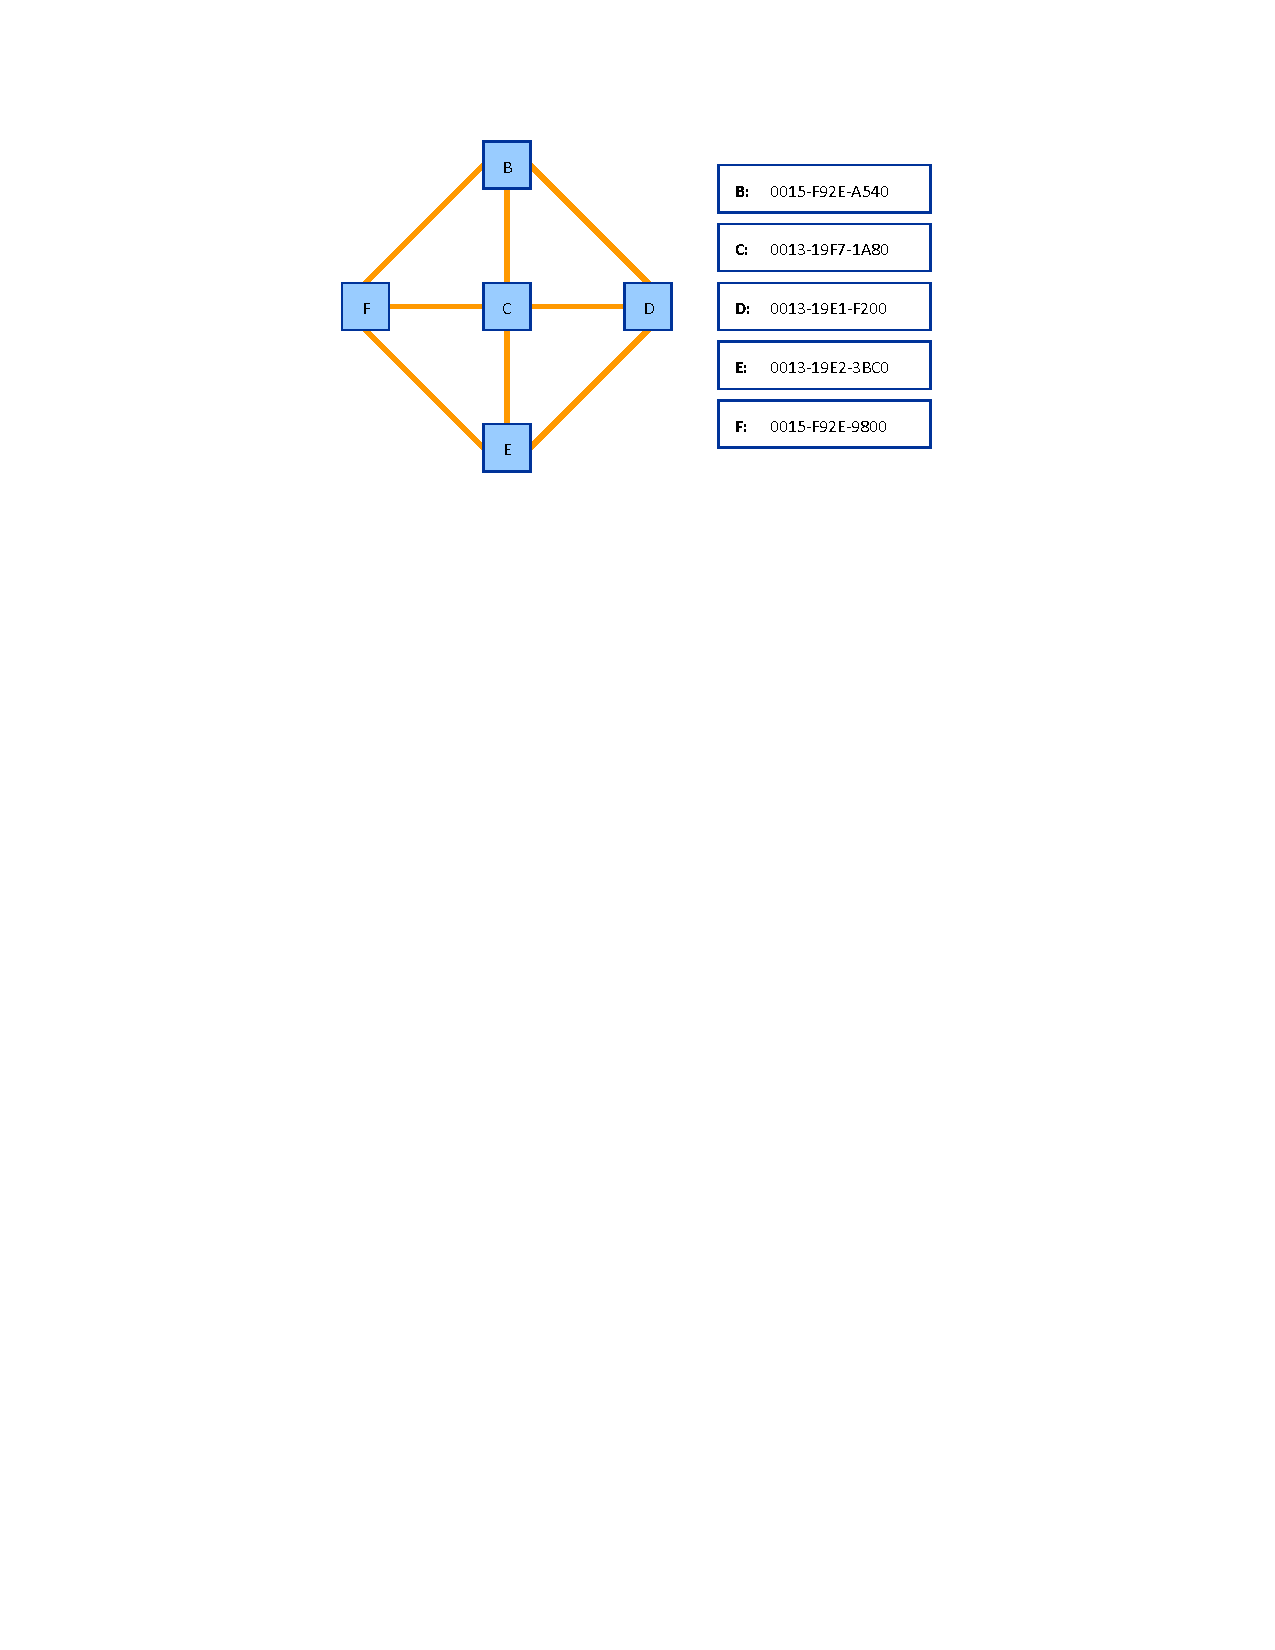
\includegraphics[width=0.9\linewidth]{Figures/StpTopology.pdf}
\else
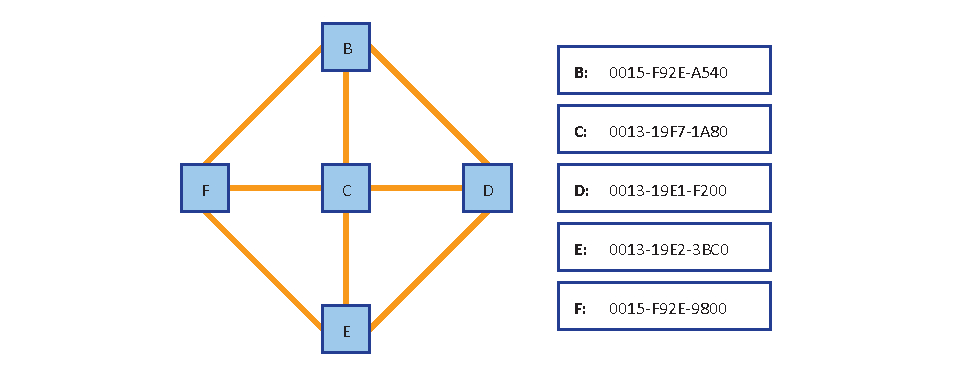
\includegraphics[width=0.9\linewidth]{Figures/StpTopology.eps}
\fi
\caption{The network topology used for the STP practical exercise.}
\label{fig:StpTopology}
\end{figure}

\begin{center}
\sffamily\small
\begin{tabular}{>{\columncolor{tablegray}}p{15cm}}

\multicolumn{1}{>{\columncolor{tableorange}}l}{Questions and Tasks}\\
Find the \texttt{\color{blue}BridgeId} of each switch.\\
\hline
Compute which is the spanning tree and draw it.\\
\hline
Which is the root switch?\\
\hline
Which is the role of each port?\\
\hline
Which are the activated ports?\\
\hline
\end{tabular}
\end{center}

Fill in the table \ref{tab:Stp}.


\begin{table}
\sffamily\small
\centering
\begin{tabular}{>{\columncolor{tablegray}}ccccc}
\multicolumn{1}{>{\columncolor{tableorange}}c}{Switch ID} & \multicolumn{1}{>{\columncolor{tableheader}}c}{MAC} & \multicolumn{1}{>{\columncolor{tableheader}}c}{Port} & \multicolumn{1}{>{\columncolor{tableheader}}c}{Role} &
\multicolumn{1}{>{\columncolor{tableheader}}c}{State} \\
Switch B & 00:15:F9:2E:A5:40 & & & \\
\hline
Switch C & 00:13:19:F7:1A:80 & & & \\
\hline
Switch D & 00:13:19:E1:F2:00 & & & \\
\hline
Switch E & 00:13:19:E2:3B:C0 & & & \\
\hline
Switch F & 00:15:F9:2E:98:00 & & & \\
\hline
\end{tabular}
\caption{The spanning tree.}
\label{tab:Stp}
\end{table}

\section{Practical Verification}

Now you will verify that the STP constructed by the switches is in fact the one you computed in the previous section. Use the VLAN 1 to connect to the five switches (B, C, D, E, F). It is recommended to open five simultaneous Telnet connections, one for each of the switch.

Each group will work in a different VLAN. The teacher will assign a VLAN to each group. Make sure that your VLAN is included in all the trunk ports. Each group will have a different STP, as the network creates a tree for each VLAN.

In each of the switches, enter the \emph{privileged EXEC} mode and use the command:

\begin{lstlisting}
Switch# show spanning-tree vlan <id>
\end{lstlisting}

Observe all the fields and make sure you understand them.

\begin{center}
\sffamily\small
\begin{tabular}{>{\columncolor{tablegray}}p{15cm}}
\multicolumn{1}{>{\columncolor{tableorange}}l}{Question}\\
What can you see?\\
\hline
Find the BridgeId of each switch. Compute which is the spanning tree and draw it.\\
\hline
Which switch is the root? Which is the role of each port? Which ports are activated?\\
\hline
Fill in the table \ref{tab:Stp} and compare practical results to the theoretical computation.\\
\hline
\end{tabular}
\end{center}



\section{Changing the STP Configuration}

Now that you are familiar with the STP parameters, you will make some changes that will result in the computation of a new tree. In the \emph{global configuration} mode use the command:

\begin{lstlisting}
Switch(config)# spanning-tree vlan <id>
\end{lstlisting}
or, alternatively, you may use:

\begin{lstlisting}
Switch(config)# interface vlan <id>
Switch(config)# spanning-tree
\end{lstlisting}
to see which parameters are susceptible to be configured. Use the question mark \texttt{\color{blue}?} to see all the available parameters and make sure you understand them.

The exercise that we propose is to change the priority of one of the switches different from the root switch. The default behavior is that the switch with the lowest MAC address is selected as a root. The reason is that, in the default configuration, the priority of all the switches is 32768. By changing the priority of one of the switches to a lower value, we can force that that particular switch becomes the root.

Go ahead and change the root switch and observe the new configuration of the tree. Fill in the table \ref{tab:Stp} for this new configuration and draw the new tree.

\section{Link Failure}

This exercise cannot be started until all the groups have finished the previous one. If you reach this exercise before the other groups, move on to the next exercise while you wait for all the groups to be ready for the link failure.

Now we will disconnect one of the links to simulate a link failure. Compute in advance your new spanning tree after the link failure. Ask your teacher which is the cable that will be disconnected.

After the disconnection, check which is the new configuration and compare it with the one that you have predicted. Explain what happened.

\section{BPDUs}

Use the computer connected to the VLAN 1 (the computer used for the administration of the switch) and capture the traffic for several seconds using \emph{Wireshark}. Observed the received STP frames and identify the different fields in the packet. Write them down to include them in your report and find out which is the meaning of the information in each of the fields.

\begin{center}
\sffamily\small
\begin{tabular}{>{\columncolor{tablegray}}p{15cm}}

\multicolumn{1}{>{\columncolor{tableorange}}l}{Question}\\
Why are you receiving these frames at your computer?\\
\hline
\end{tabular}
\end{center}
